\documentclass[a4paper,11pt]{article}
\usepackage{amsmath,amsthm,amsfonts,amssymb,amscd,amstext,vmargin,graphics,graphicx,tabularx,multicol} \usepackage[french]{babel}
\usepackage[utf8]{inputenc}  
\usepackage[T1]{fontenc} 
\usepackage[T1]{fontenc}
\usepackage{amsmath,amssymb}
\usepackage{pstricks-add,tikz,tkz-tab,variations}
\usepackage[autolanguage,np]{numprint} 
\usepackage{color}
\usepackage{ulem}

\setmarginsrb{1.5cm}{0.5cm}{1cm}{0.5cm}{0cm}{0cm}{0cm}{0cm} %Gauche, haut, droite, haut
\newcounter{numexo}
\newcommand{\exo}[1]{\stepcounter{numexo}\noindent{\bf Exercice~\thenumexo} : \marginpar{\hfill /#1}}
\reversemarginpar


\newcounter{enumtabi}
\newcounter{enumtaba}
\newcommand{\q}{\stepcounter{enumtabi} \theenumtabi.  }
\newcommand{\qa}{\stepcounter{enumtaba} (\alph{enumtaba}) }
\newcommand{\initq}{\setcounter{enumtabi}{0}}
\newcommand{\initqa}{\setcounter{enumtaba}{0}}

\newcommand{\be}{\begin{enumerate}}
\newcommand{\ee}{\end{enumerate}}
\newcommand{\bi}{\begin{itemize}}
\newcommand{\ei}{\end{itemize}}
\newcommand{\bp}{\begin{pspicture*}}
\newcommand{\ep}{\end{pspicture*}}
\newcommand{\bt}{\begin{tabular}}
\newcommand{\et}{\end{tabular}}
\renewcommand{\tabularxcolumn}[1]{>{\centering}m{#1}} %(colonne m{} centrée, au lieu de p par défault) 
\newcommand{\tnl}{\tabularnewline}

\newcommand{\trait}{\noindent \rule{\linewidth}{0.2mm}}
\newcommand{\hs}[1]{\hspace{#1}}
\newcommand{\vs}[1]{\vspace{#1}}

\newcommand{\N}{\mathbb{N}}
\newcommand{\Z}{\mathbb{Z}}
\newcommand{\R}{\mathbb{R}}
\newcommand{\C}{\mathbb{C}}
\newcommand{\Dcal}{\mathcal{D}}
\newcommand{\Ccal}{\mathcal{C}}
\newcommand{\mc}{\mathcal}

\newcommand{\vect}[1]{\overrightarrow{#1}}
\newcommand{\ds}{\displaystyle}
\newcommand{\eq}{\quad \Leftrightarrow \quad}
\newcommand{\vecti}{\vec{\imath}}
\newcommand{\vectj}{\vec{\jmath}}
\newcommand{\Oij}{(O;\vec{\imath}, \vec{\jmath})}
\newcommand{\OIJ}{(O;I,J)}

\newcommand{\bmul}[1]{\begin{multicols}{#1}}
\newcommand{\emul}{\end{multicols}}


\newcommand{\reponse}[1][1]{%
\multido{}{#1}{\makebox[\linewidth]{\rule[0pt]{0pt}{20pt}\dotfill}
}}

\newcommand{\titre}[5] 
% #1: titre #2: haut gauche #3: bas gauche #4: haut droite #5: bas droite
{
\noindent #2 \hfill #4 \\
#3 \hfill #5

\vspace{-1.6cm}

\begin{center}\rule{6cm}{0.5mm}\end{center}
\vspace{0.2cm}
\begin{center}{\large{\textbf{#1}}}\end{center}
\begin{center}\rule{6cm}{0.5mm}\end{center}
}



\begin{document}
\pagestyle{empty}
\titre{Interrogation 2 : Transformations}{Nom}{Prénom}{Date}{Classe}


\vspace*{0.5cm}

\exo{4} Un pavage du rectangle IJKL ci-dessous est réalisé par 24 pièces superposables $\epsilon$ dont la forme est précisée ci-après. Ces pièces sont numérotées de 1 à 24.

\bmul{2}

\begin{flushleft}
\includegraphics[scale=0.9]{exotranf7.eps} 
\end{flushleft}

\columnbreak

\initq \q Quelle est l'image de la pièce 1 par la symétrie d'axe (AB) ?\\
\reponse[2]\\
\q Quelle est l'image de la pièce 4 par la symétrie de centre B ?\\
\reponse[2]\\


\emul

\q Quelle est l'image de la pièce 3 par la translation qui transforme C en B  ?\\
\reponse[1]\\

\q Quelle est l'image de la pièce 8 par la rotation de centre B et d'angle 90\degre dans le sens des aiguilles d'une montre ?\\
\reponse[1]\\

\vspace*{0.25cm}

\exo{2} Le trapèze KLMN est l'image du trapèze ABCD par une translation.

\begin{center}
\includegraphics[scale=0.7]{exotranf6.eps} 
\end{center}

\initq 

\q  Caractériser cette translation par une flèche sur le sujet.\\

\q Déterminer la mesure de l'angle $\widehat{KLM}$. \textit{Justifier}.\\
\reponse[2]\\

\q Déterminer la distance LM. \textit{Justifier}.\\
\reponse[2]\\

\newpage

\vspace*{0.5cm}

\exo{4} Sur le quadrillage ci-dessous, effectuer les constructions suivantes :\\
- en bleu l'image du polygone BCDEFG par la rotation de centre G et d'angle 90\degre dans le sens antihoraire ;\\
- en rouge l'image du polygone BCDEFG par la translation qui transforme G en C ;\\
- en vert l'image du polygone BCDEFG par la symétrie d'axe (d);\\
- en noir l'image du polygone BCDEFG par la symétrie centrale de centre W.\\

\vspace*{0.5cm}

\includegraphics[scale=0.9]{bilan.eps} 


\vspace*{1cm}

\exo{+1,5} \textit{BONUS}\\
Construire la suite de cette frise en construisant l'image du motif par la translation définie par la flèche du
bas puis construire la suite en construisant l'image de la figure par la translation définie par la flèche du haut.

\begin{flushleft}
\includegraphics[scale=0.75]{pavage.eps} 
\end{flushleft}


\end{document}
